\section{Materials and Methods}

\subsection{Study 1: Evaluateion bias and variance of cross-validation}

This study investigated the interplay between sample size and various performance estimators and their collective impact on bias and variance during model validation. It is hypothesized that increasing the sample size will reduce both bias and variance. Additionally, it is expected that the validation variance will increase with the number of folds in the CV, while simultaneously reducing bias. Since K-fold CV employs a fraction (i.e., $K-1$ folds) of the data for training, it may provide a pessimistic estimate of model performance. Hence, this study designed to assess the underestimation from each performance estimators, including K-fold CV with K set to 2, 5, and 10, as well as LOOCV where K equals the sample size N, and the "In-Sample" evaluation, which assesses model performance on the same dataset used for training, potentially leading to an overly optimistic bias. To gauge model performance, three metrics are employed: RMSE (Eq. ~\ref{eq_rmse}), r (Eq. ~\ref{eq_r}), and $R^2$ (Eq. ~\ref{eq_R2}). The validation model is a multivariate linear regression with ten input features and one output target, all drawn from a standard normal distribution $\mathcal{N}(0, 1)$, implying no expected linear relationship between inputs and the target, with an expected correlation r of zero. The sample sizes N are varied among 50, 100, and 500 to explore the dynamics between sample size and performance estimators. Each configuration is repeated across 1000 iterations to assess the distribution of bias and variance.

For each iteration, the dataset $\mathcal{D}={(X, Y)}$ was sampled as per the simulation’s premise. In the case of K-fold CV, the dataset $\mathcal{D}$ was partitioned into K folds in which each fold is $\mathcal{D}_k={(X_k, Y_k)}$. For the “In-Sample” approach, partitioning does not occur. The linear model f is trained on the training set $\mathcal{D}_\text{-k}$ (denoted as $f_{\mathcal{D}_{\text{-k}}}$) to estimate regression coefficients $\beta$, which then predicts the target variable ${\hat{Y}}_k$ from the test set $\mathcal{D}_k$. The procedure of K-fold CV can be expressed as:


\begin{equation} \label{eq_kfoldcv}
    \begin{split}
	\text{Training: } \quad Y_{\text{-k}} &= f_{\mathcal{D}_{\text{-k}}}(X_{\text{-k}})+\epsilon \\
    &= X_{\text{-k}} \beta + \epsilon \\
    \text{Testing: } \quad \hat{Y}_k &= f_{\mathcal{D}_{\text{-k}}}(X_k) \\
    &=X_k \beta \quad \quad \quad k=1,2,\ldots,K
    \end{split}
\end{equation}

For the “In-Sample” performance estimator, predictions were made without splitting, as:

\begin{equation} \label{eq_insample}
    \begin{split}
    	\text{Training: } \quad Y &= f_\mathcal{D}(X) \\ &= X\beta + \epsilon \\
        \text{Testing: } \quad \hat{Y} &= f_\mathcal{D}(X) \\ &=X \beta
    \end{split}
\end{equation}

Where:
\begin{itemize}
  \item \( X \) denotes the input regressors sampled from a standard normal distribution \( \mathcal{N}(0, 1) \) with dimensions \( N \times 10 \).
  \item \( Y \) denotes the target variable sampled from a standard normal distribution \( \mathcal{N}(0, 1) \) with dimensions \( N \times 1 \).
  \item \( X_\text{-k} \) and \( Y_\text{-k} \) are the input regressors and target variable in the training set \( \mathcal{D}_\text{-k} \).
  \item \( X_k \) denotes the input regressors in the test set \( \mathcal{D}_k \).
  \item \( \hat{Y}_k \) denotes the predicted target variable in the test set \( \mathcal{D}_k \).
  \item \( \beta \) denotes the estimated regression coefficient with dimensions \( 10 \times 1 \).
  \item \( \epsilon \) denotes the error term assumed to be normally distributed.
\end{itemize}

Estimated performance $\mathbb{E}[\hat{g}(f_\mathcal{D})]$ was derived by averaging the performance metrics across all K folds as per Eq. ~\ref{eq_g_exp}. The bias and variance of the evaluation were calculated using Eqs. ~\ref{eq_bias} and ~\ref{eq_var}, respectively. To approximate true model performance $G(f_\mathcal{D})$, a hundred unseen datasets $\mathcal{D}^\ast$ were generated identically to $\mathcal{D}$, and the performance $G(f_\mathcal{D})$ was estimated by averaging the performance metrics across all $\mathcal{D}^\ast$. The detailed steps to compute evaluation bias and variance are provided in the supplementary materials.

\subsection{Study 2: Model Selection in Cross-Validation}

The objective of this simulation study is to examine the effect of improper model selection implementation on validation bias. The focus will be on the model selection procedures of feature selection and hyperparameter tuning. The study hypothesizes that utilizing the test set inappropriately during any model selection stage will lead to a significant overestimation of model performance. This study simulated a regression task using an SVR model, which utilized various kernel functions to project a subset of features, X, to predict a target variable, Y. Both X and Y are drawn from a normal distribution $\mathcal{N}(0, 1)$ to establish a baseline null correlation (performance r=0) for assessing validation bias. This study set the sample size and number of features at 100 and 1000, respectively. Feature selection is executed by choosing the top 50 features that correlate most strongly with Y. For hyperparameter tuning, four kernel functions were evaluated: linear, polynomial, radial basis function, and sigmoid.
\begin{figure}[h]
    \centering
    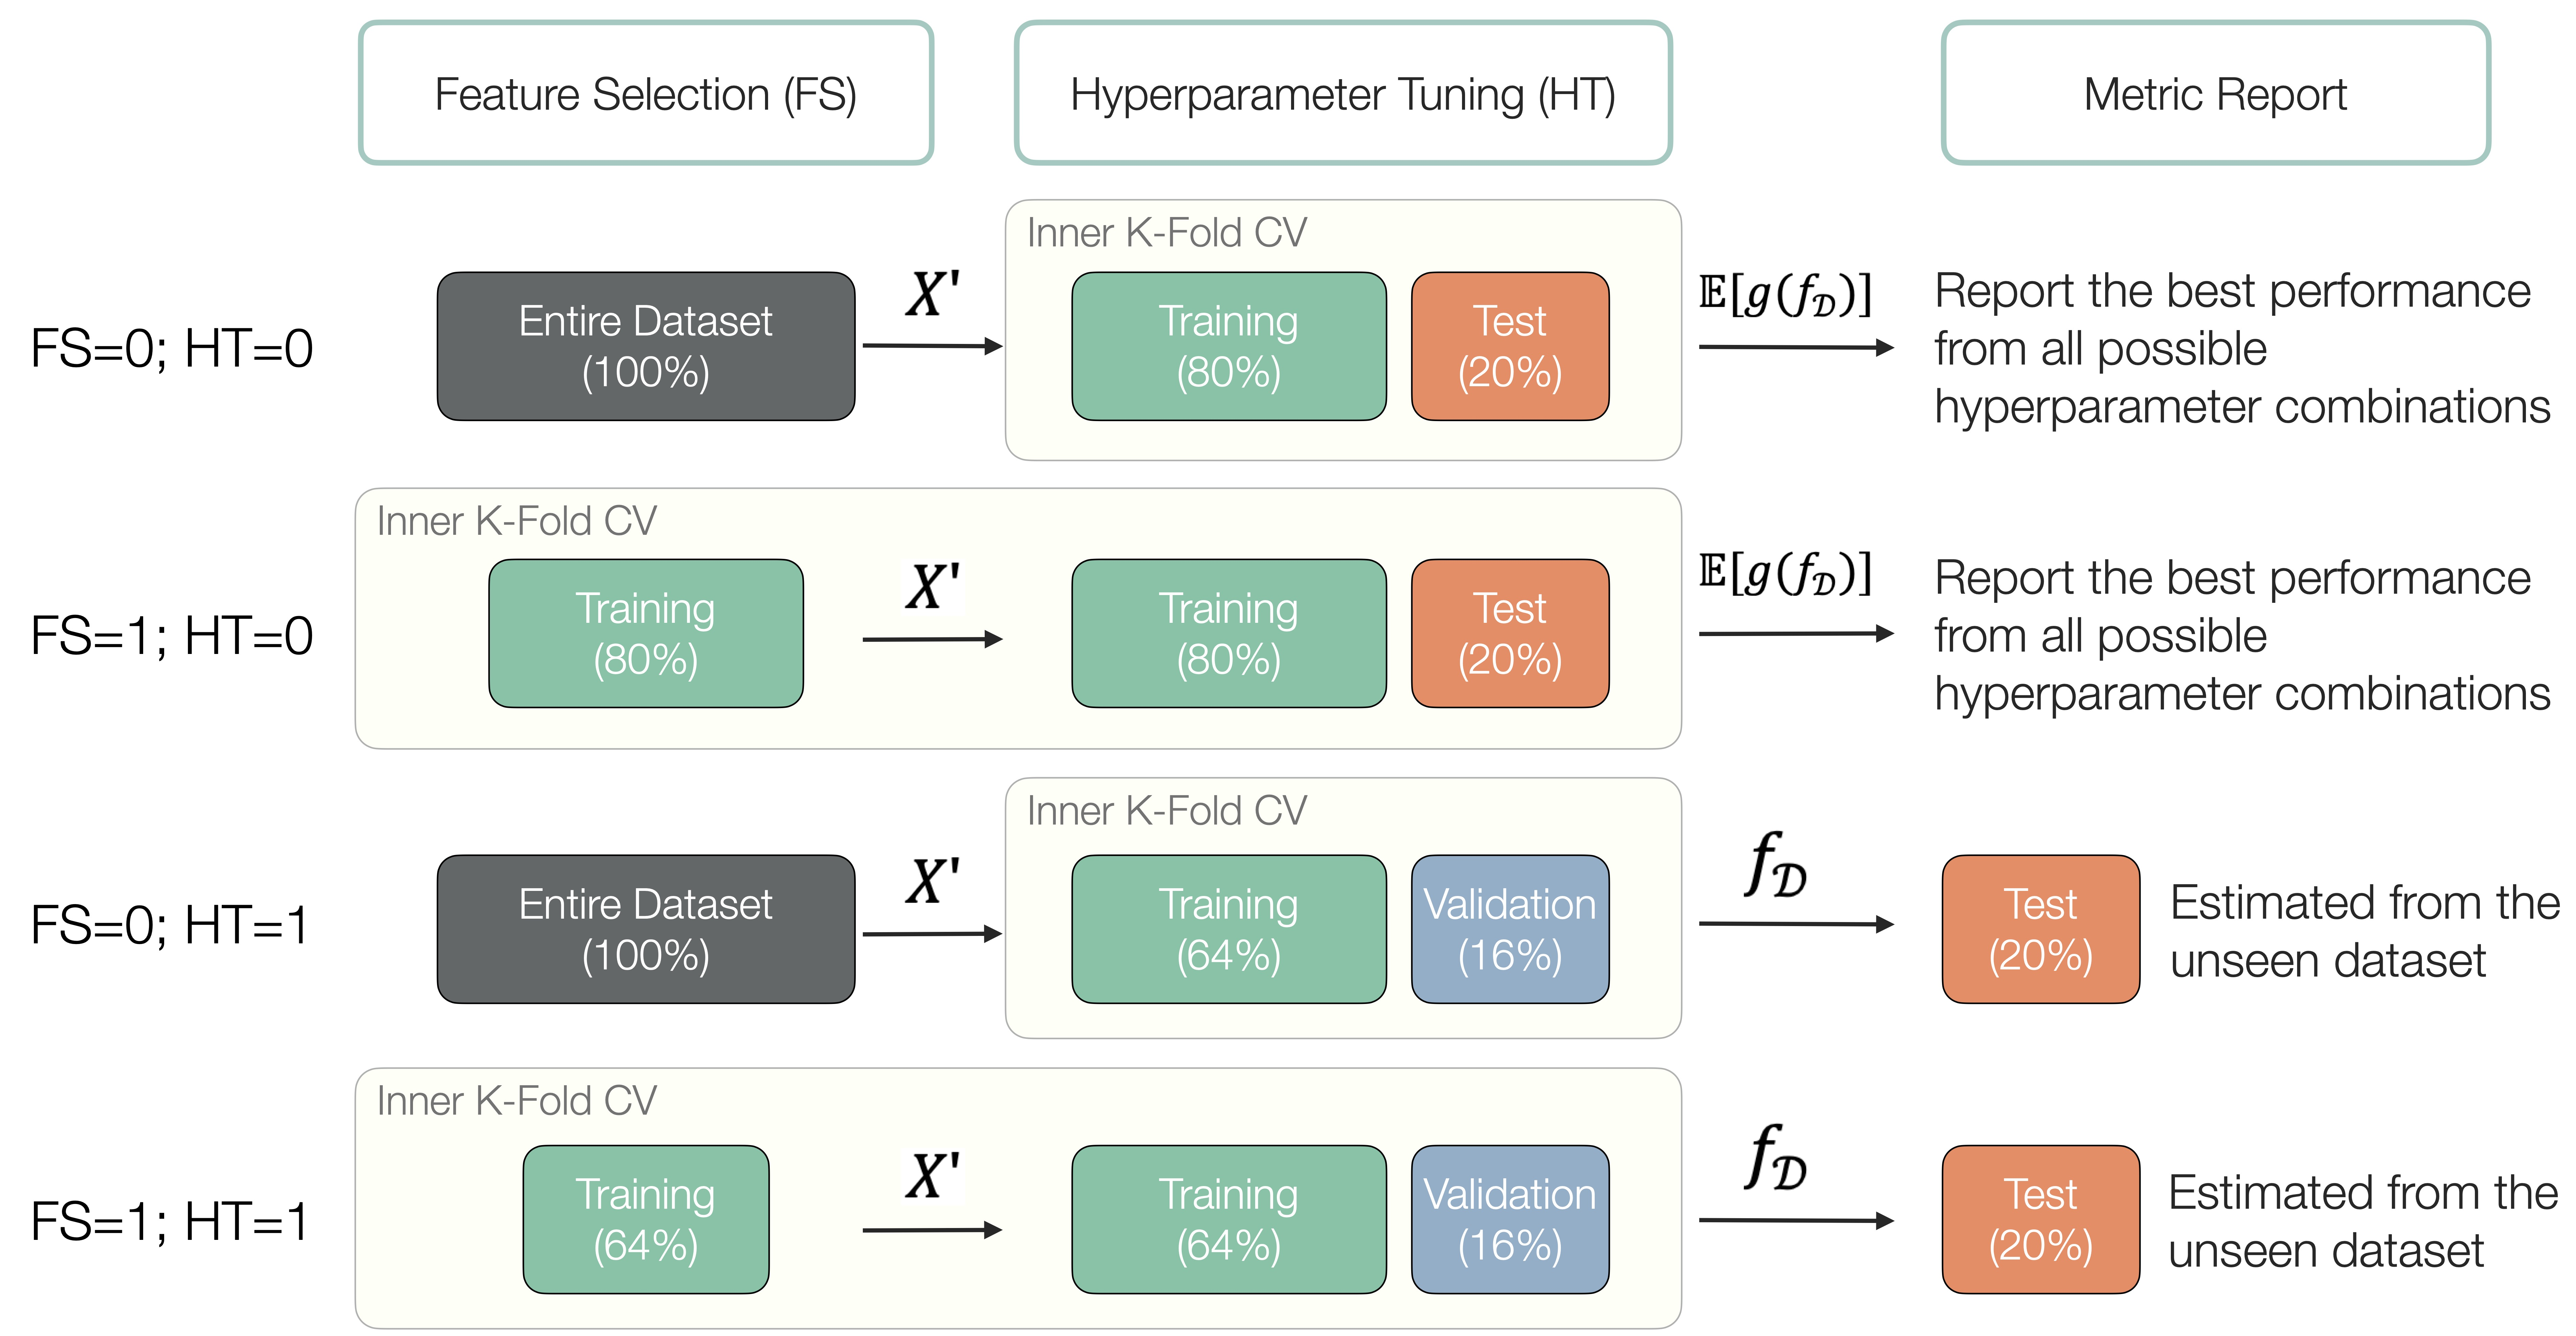
\includegraphics[width=1\textwidth]{fig_s2_schemes.jpg}
    \caption{Workflow diagram illustrating four cross-validation strategies of feature selection (FS) and hyperparameter tuning (HT), where 0 denotes incorrect implementation and 1 indicates correct practice. $X'$ is the selected feature subset, $\mathbb{E}[\hat{g}(f_\mathcal{D})]$ is the expected generalization performance, $f_\mathcal{D}$ is the model trained on the training set without being revealed to the test set.}
    \label{fig:s2_schemes}
\end{figure}

This study introduces notations FS for feature selection and HT for hyperparameter tuning, assigning a binary indicator (0 or 1) to denote incorrect (0) or correct (1) implementation of model selection. This yields four possible combinations of model selection strategies: “FS=0; HT=0”, “FS=0; HT=1”, “FS=1; HT=0”, “FS=1; HT=1” (Figure ~\ref{fig:s2_schemes}). When FS=0, feature selection precedes cross-validation splitting. If FS=1, feature selection occurs within each fold of the training set during cross-validation. With hyperparameter tuning, a correct implementation (HT=1) involves splitting the dataset into training (64\%), validation (16\%), and test (20\%) sets. The model is trained and tuned using the training and validation sets, respectively, while the test set is reserved for a single evaluation of model performance. Conversely, with HT=0, only training (80\%) and test (20\%) sets are used, risking validation bias as the test set informs both training and performance reporting. A 5-fold cross-validation approach was deployed for all strategies.
Validation bias is measured as the discrepancy between the model selection-influenced performance estimate and the expected generalization performance (r=0), using the Pearson correlation coefficient between predicted and observed values. Over 1000 sampling iterations, the study assesses the distribution of validation bias. A t-test will determine whether the validation bias significantly deviates from zero.

\subsection{Study 3: Block Effects in Cross-Validation}

The objective of the study is to demonstrate how a Random CV, which randomly assigns the samples to folds without considering the block effects, could overestimate the model performance. This study also conducts a block CV, where each block is used as a fold in the cross-validation, as the benchmark. The hypothesis is that the model performance estimated by Random CV is significantly higher than the estimation by block CV. This study simulated a regression task with 100 instances across ten features, denoted as X, and one single response variable, Y. Both X and Y are derived from a standard normal distribution. To introduce a block factor, the study groups every 20 observations into a block, with each block incrementally increasing by b units from zero, where b was simulated from 0.5 to 3.0 with an increment of 0.5. Within these ten features, one is substituted as the block level, represented by an integer from 0 to 4, augmented with random noise drawn from a standard normal distribution. This setup aims to simulate a scenario where the predictors primarily capture block variation, given the null expectation in predictability when using ten random variables X to forecast another random variable Y.
The study investigates two model validation strategies: Block CV and Random CV, both utilizing a 5-fold cross-validation method. In block CV, each block serves as a separate fold, while in Random CV, samples are randomly allocated to each fold (Figure ~\ref{fig:s3_block}). The predictive model is linear regression, and the performance is evaluated using Pearson's correlation coefficient. This simulation runs for 1000 iterations, with X and Y being resampled in each cycle. A one-tailed t-test assesses if the mean estimated performance significantly exceeds zero. Additionally, an Analysis of Variance (ANOVA) table is calculated when b is 0.5 to ascertain if the simulated block variation notably exceeds the assumed individual variation, representing the primary interest.

\begin{figure}[h]
    \centering
    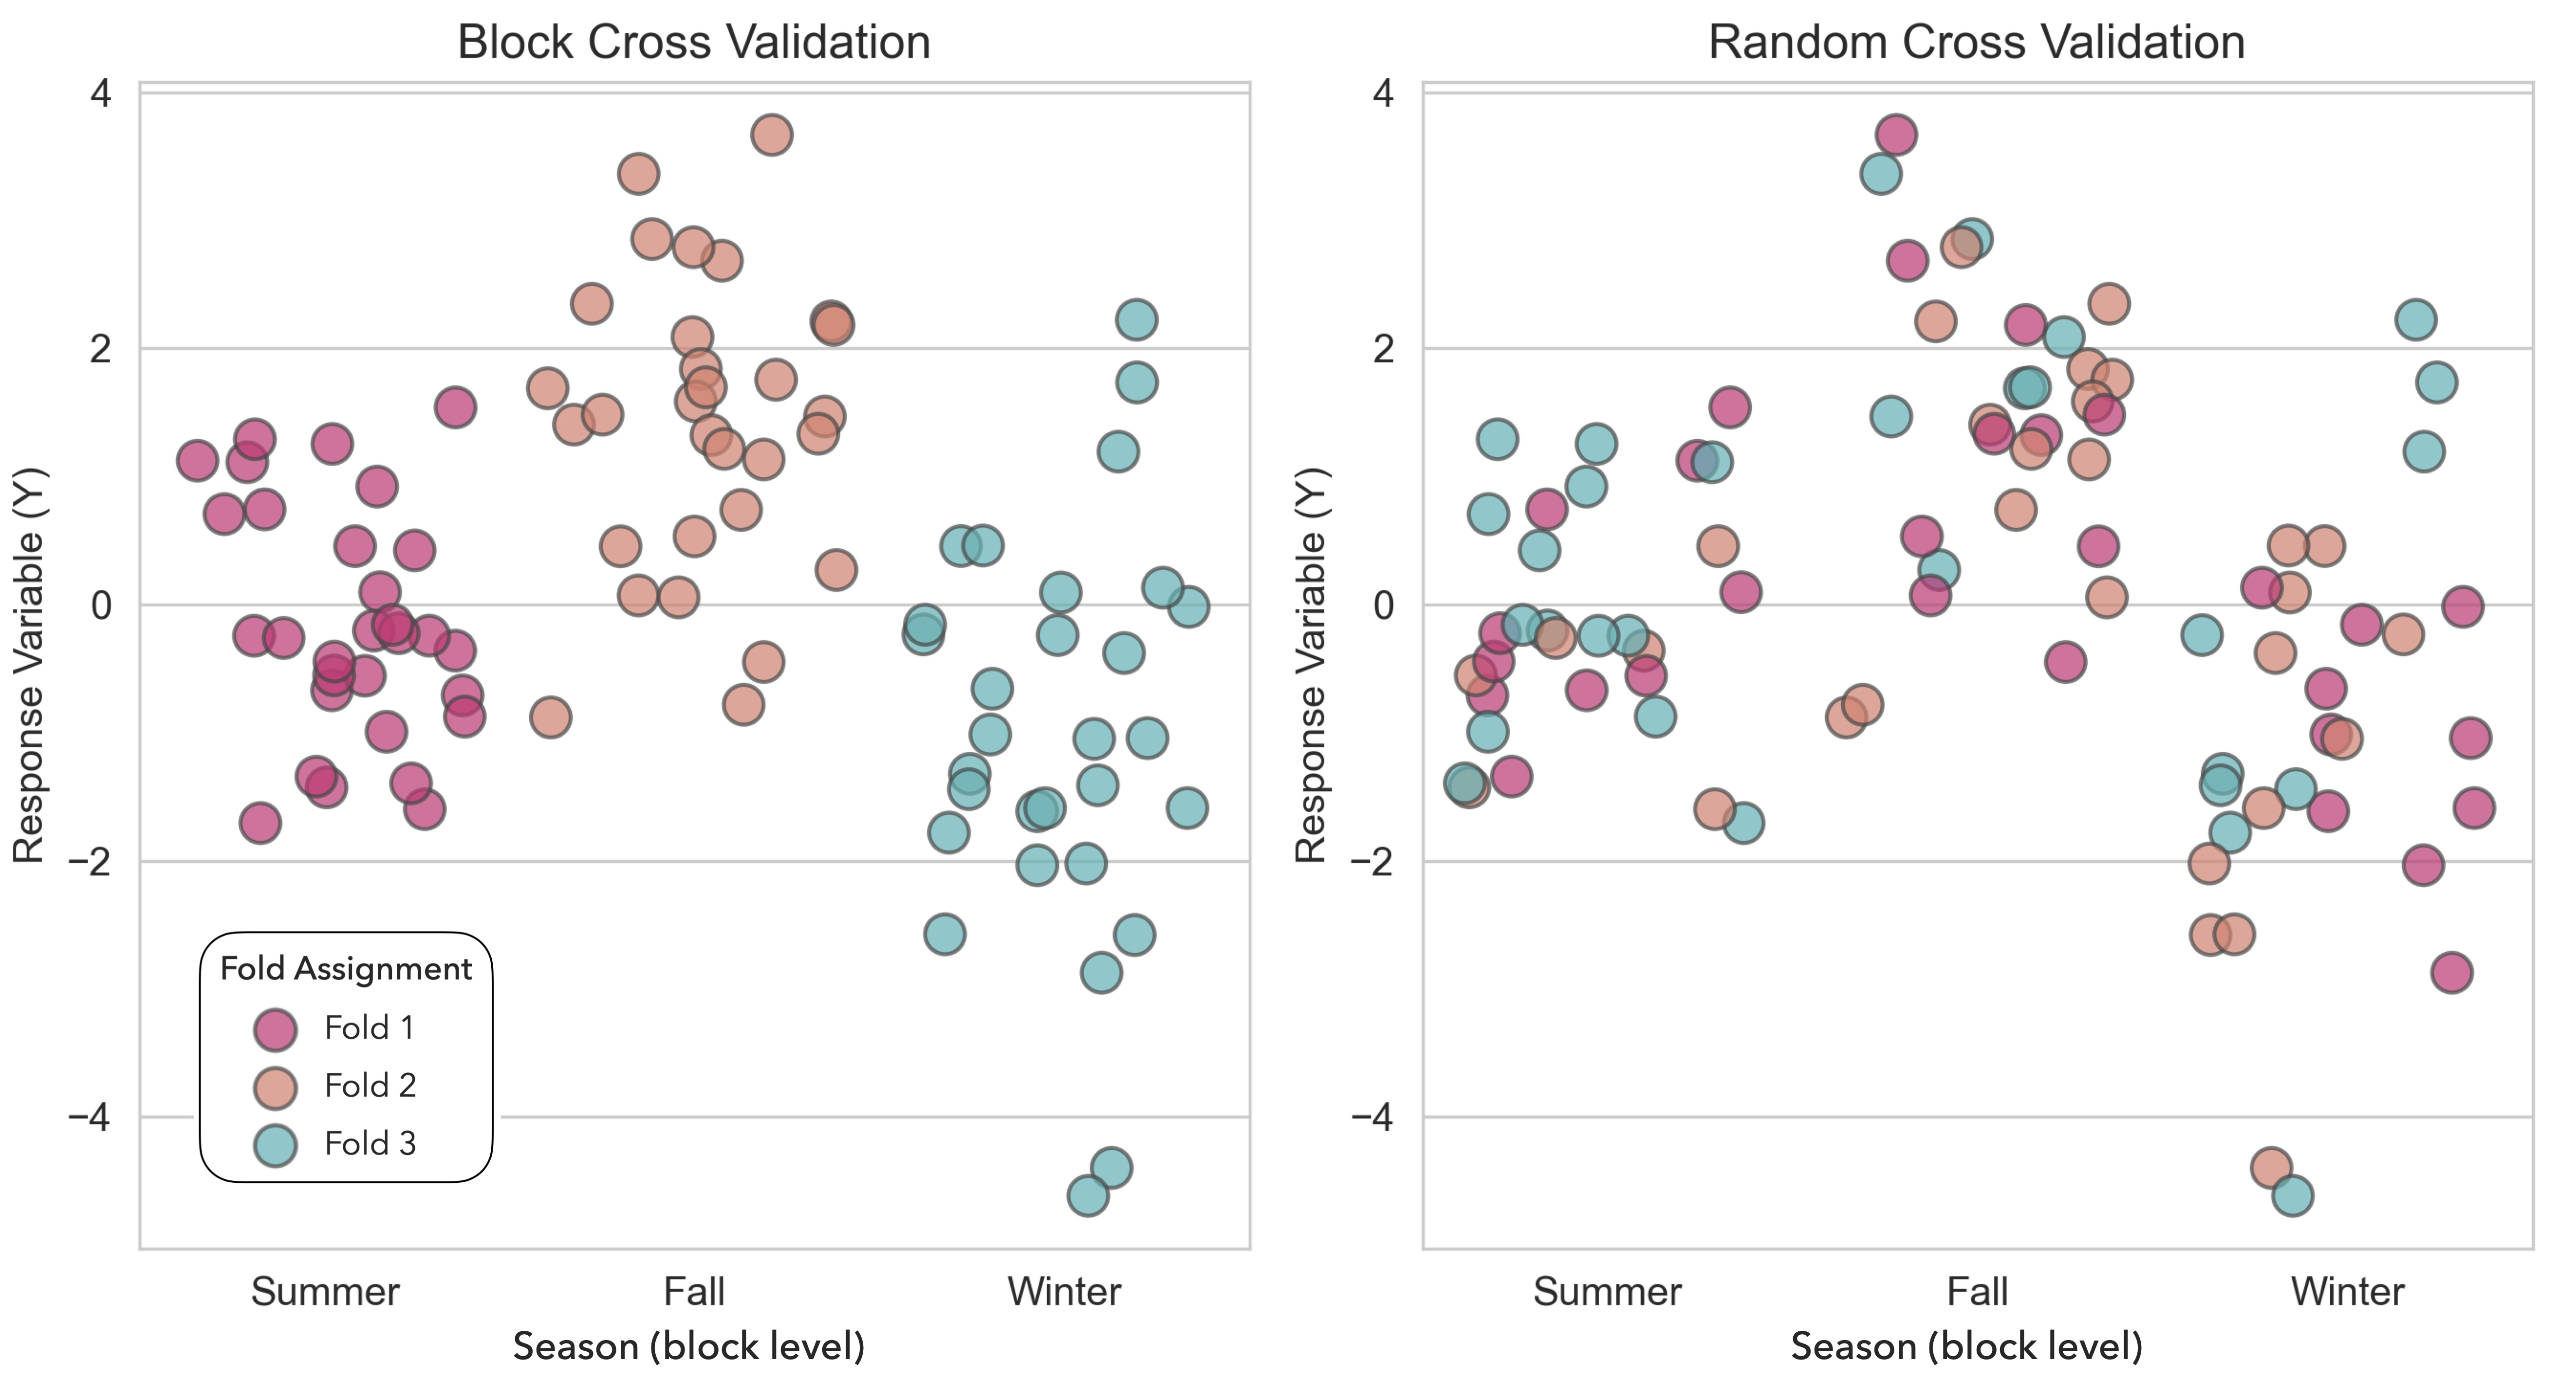
\includegraphics[width=1\textwidth]{fig_s3_block.jpg}
    \caption{Illustration of fold assignment in block cross validation (left) and random cross validation (right). Folds are color-coded, and the block effect is set to 3 in this example.}
    \label{fig:s3_block}
\end{figure}

\subsection{Study 4: Performance Metrics in Regression Tasks}

This study explores two error-based metrics, Root Mean Squared Error (RMSE) and Root Mean Squared Percentage Error (RMSPE), and three linearity-based metrics, 
Pearson Correlation Coefficient ($r$), the Coefficient of Determination ($R^2$), and the Concordance Correlation Coefficient ($CCC$), in a variety of commonly-encountered data challenges. These data challenges are depicted through 4 scenarios, representing data commonly encountered in predictive applications varying in scope (scenarios 1 and 2), data with outliers disrupting the scale of prediction (scenario 3), and data with an underlying grouping structure (scenario 4). The statistical description of the approach to generating each of these scenarios is included below. Practical examples of real-world instances of these types of data challenges are also described.

In the hypothetical example depicted in Figure ~\ref{fig:s4_reg}, 100 observations were generated from two separate normal distributions. The first 50 observations were drawn from a normal distribution with a mean of -3 and a standard deviation of 1, denoted as $\mathcal{N}(-3, 1)$. The remaining 50 observations were generated from another normal distribution, $\mathcal{N}(3, 1)$. Utilizing two distinct distributions served to simulate experimental block effects, preset at a magnitude of 6 units for this experiment. Based on the simulated observations, four scenarios of predictions were derived according to the setting below:

\begin{itemize}
    \item Scenario 1: To establish a correlation relationship, the observations were multiplied by 0.3, followed by the addition of random noise $\mathcal{N}(0, 0.7)$ to introduce prediction errors. This scenario represents a “best case” for developing predictive analytics, and could be exemplary of scenarios like predicting a scaled performance response (i.e., milk yield, average daily gain) from measurable input variables like dry matter intake, sensor system data, or past performance data.
	\item Scenario 2: The prediction outcome from Scenario 1 was multiplied by 5, simulating predictions with a larger variance while maintaining the same relative order as the original predictions. There are some responses that have naturally greater proportional variation compared with others. For example, an animal’s body core temperature is unlikely to vary by more than 5\%; however, daily variation around measurements like feed intake can range upwards of 30 to 40\%. Comparison of scenarios 1 and 2 explore how this natural variation should be included in interpreting predictive analytics.
	\item Scenario 3: only the top 10\% of predictions that deviate the most from zero in Scenario 1 were raised to the power of 5. The rest of the predictions were set to zero. This scenario simulates a prediction that focuses solely on the extreme samples. In disciplines like nutritional exploration, the emphasis of predictive analytics typically focuses on understanding the mean animal or the mean response of an individual animal; however, in predictive analytics focused on health or genetic merit, the emphasis of prediction is often on the extreme observations. Analytics to understand the extreme observations is always complicated by the question of whether extremes are due to true outliers or some sort of measurement error. As precision livestock farming advances, the opportunities for measurement error due to erroneous sensor measurements increases.
	\item Scenario 4: Values sampled from two normal distributions, $\mathcal{N}(-3,\ 1)$ and $\mathcal{N}(3, 1)$, were added respectively to the predictions made in Scenario 1 of Block A (colored orange in Figure 1) and Block B (colored green in Figure 1). In the animal sciences we often rely on blocks as an experimental tool to support analytics given challenging experimental design or constrained animal units. Many times, the difference between blocks dwarfs the differences observed within a block, resulting in a masking of true effects due to the block influence. This scenario amplified the original block effects, simulating a model that effectively distinguished between different blocks (e.g., herd or breed) but was less capable of predicting individual variations within each block. An example of this scenario might be simulating milk production or body weight across species – the magnitude of the difference between sheep and cattle (for example) far outweighs the magnitude of the difference of sheep or cattle over time.
\end{itemize}
This quartet of predictions serves to simulate potential challenges and complexities encountered in real-world modeling scenarios, thereby providing a foundation for evaluating different performance metrics used in regression problems.

\subsection{Study 5: Performance Metrics in Classification Tasks}

This study presents a hypothetical example to highlight how the choice of different performance metrics can lead to different interpretations of a model's effectiveness. The example focuses on binary classification, where the outcome is either positive (Y=1) or negative (Y=0). Suppose a binary classification model always outputs a probability between 0 and 1, indicating the likelihood that a sample belongs to the positive class. This example assumes that the model has high confidence in correctly predicting 1 out of 4 positive and 5 out of 6 negative samples. This example intends to illustrate a scenario where the positive outcome is rare, such as predicting the onset of a calving event in dairy cows \citep{ouellet_evaluation_2016,borchers_machine-learning-based_2017}. The example data is shown in Figure ~\ref{fig:s5_cls}. In addition to the original labels, this example also examines a scenario with inverted labels (Figure ~\ref{fig:s5_cls}. Upper). Since most classification metrics prioritize positive samples, it is generally advisable to designate the event of interest as the positive class in binary classification problems. Inverting the labels illustrates the potential overestimation of model performance when the more common, but less significant, background event is mistakenly marked as the positive class. It is important to note that inverting the labels in this example only affects the interpretation of model performance, not the model configuration or parameters.
To evaluate classification performance, one must first establish a confidence threshold to dichotomize the prediction probabilities. For instance, if a prediction probability exceeds the threshold, the sample is labeled positive. By default, the threshold is set at 0.5 for its simplicity. For example, in the third data row of the example data: With a prediction probability of 0.38 that falls below the threshold, the sample is deemed negative, resulting in a false negative classification since the ground truth is positive. It is worth mentioning that this threshold is adjustable to fine-tune model performance for particular uses. A confusion matrix (Figure ~\ref{fig:s5_cls}. Lower), effectively encapsulates prediction outcomes. The rows in this 2x2 matrix correspond to ground truth, while its columns reflect predictions. Correct predictions populate the diagonal cells, and errors fill the off-diagonal ones. This matrix serves as the foundation for computing various metrics to assess model performance, which will be explored in the result sections.

